% 실험16 E — Gated Late Fusion (위험점수 수준 gate, fig1_late_fusion_overview 레이아웃을 따름).
%   Left  : Gated Cox combiner 내부 (z_tab, z_img -> gate g_m = 2 sigma(c_m . z) -> risk = sum beta_m g_m z_m)
%   Right : 전체 모델 (Stage 1 두 arm 독립 학습 -> z-score -> Stage 2 gated stacking on inner OOF)
% 수치 출처: experiments/실험16_GMU_nestedCV/nested_fusion/{model.py (GatedLateFusion), config.py (GATED_LATE_LAMBDAS, ENCODERS)},
%            outputs/gmu_nested/run_v2_os/experiment_config.json (임상 19변수: rt_type·atezolizumab 제외).
\documentclass[tikz,border=6pt]{standalone}
% 논문 그림 공통 스타일 (fig1/fig2 가 \input 한다).
% 시각 언어는 Mixture-of-Recursions(MoR) 논문 Fig.1/2 를 따른다:
%   파스텔 채움 + 진남색 얇은 윤곽 + 둥근 모서리, 산세리프 라벨.
% 색 의미(두 그림에서 동일):
%   boxblue   = 영상 모달리티      boxpurple = 임상 모달리티     boxpink = 판독지 모달리티
%   boxgray   = 일반 연산 블록     boxyellow = Cox 관련(head/combiner)
%   dashed    = 동결(frozen) 사전학습 모듈
\usepackage[T1]{fontenc}
\usepackage{helvet}
\renewcommand{\familydefault}{\sfdefault}
\usepackage{amsmath,amssymb}
\usetikzlibrary{positioning,arrows.meta,calc,fit,backgrounds}

\definecolor{navy}{HTML}{2F3B52}
\definecolor{ink}{HTML}{1A1A1A}
\definecolor{ink2}{HTML}{5A5E66}
\definecolor{boxblue}{HTML}{CFE0F7}
\definecolor{boxpink}{HTML}{F6CDD0}
\definecolor{boxpurple}{HTML}{DCD6F3}
\definecolor{boxyellow}{HTML}{FDEEB8}
\definecolor{boxgray}{HTML}{E9E9E9}
\definecolor{cellhold}{HTML}{3F5A8A}
\definecolor{cellfit}{HTML}{F8DD8A}
\definecolor{celleval}{HTML}{F2A4A8}

\tikzset{
  every node/.style={text=ink},
  blk/.style={draw=navy, line width=0.7pt, rounded corners=2.5pt, fill=#1,
              inner xsep=4pt, inner ysep=3pt, font=\footnotesize, align=center},
  blk/.default=boxgray,
  lay/.style={blk=#1, minimum width=30mm, minimum height=6mm},
  inp/.style={blk=#1, minimum width=15mm, minimum height=7mm},
  frozen/.style={lay=boxgray, dashed},
  container/.style={draw=navy, line width=0.8pt, rounded corners=6pt, fill=white, inner sep=6pt},
  armbox/.style={draw=navy, line width=0.6pt, dashed, rounded corners=5pt, inner sep=4pt},
  arr/.style={-{Latex[length=2.2mm,width=1.7mm]}, draw=navy, line width=0.75pt},
  lab/.style={font=\scriptsize, text=ink2, align=center, inner sep=1pt},
  op/.style={circle, draw=navy, line width=0.7pt, fill=white, inner sep=0pt,
             minimum size=4.2mm, font=\scriptsize},
  risk/.style={font=\footnotesize, inner sep=2pt},
  stage/.style={font=\scriptsize\itshape, text=ink2, inner sep=1pt},
  ptitle/.style={font=\footnotesize, align=center, inner sep=2pt},
}

% ---------------------------------------------------------------------------
% 입력 모달리티 아이콘 (fig2 입력단). 글자 라벨 대신 실제 PET-CT MIP 한 장 +
% 임상 표 / 판독지 문서 픽토그램을 쓴다. 모두 약 10.5mm x 12mm 로 크기를 맞추고
% 채움색은 모달리티 색(boxblue/boxpurple/boxpink), 윤곽은 navy 로 본문 도형과 통일.
%   사용: \iconimage{노드이름}{(x,y)}  등. 노드이름으로 화살표를 걸 수 있다.
\newcommand{\iconimage}[2]{%
  \node[blk=boxblue, inner sep=1.1pt, minimum width=0pt, minimum height=0pt] (#1) at #2
       {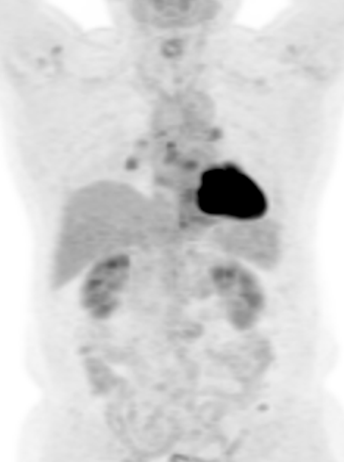
\includegraphics[height=11.8mm]{assets/pet_mip_icon.png}};%
}
\newcommand{\iconclinical}[2]{%
  \begin{scope}[shift={#2}]
    \begin{scope}
      \clip[rounded corners=2.5pt] (-5.25mm,-6mm) rectangle (5.25mm,6mm);
      \fill[boxpurple] (-5.25mm,-6mm) rectangle (5.25mm,6mm);
      \fill[navy!28]   (-5.25mm,3.3mm) rectangle (5.25mm,6mm);
      \draw[navy!45, line width=0.35pt]
        (-5.25mm,3.3mm) -- (5.25mm,3.3mm)  (-5.25mm,0.8mm) -- (5.25mm,0.8mm)
        (-5.25mm,-1.7mm) -- (5.25mm,-1.7mm) (-5.25mm,-4.2mm) -- (5.25mm,-4.2mm)
        (-1.75mm,-6mm) -- (-1.75mm,6mm)     (1.75mm,-6mm) -- (1.75mm,6mm);
    \end{scope}
    \draw[navy, line width=0.7pt, rounded corners=2.5pt] (-5.25mm,-6mm) rectangle (5.25mm,6mm);
    \node[minimum width=10.5mm, minimum height=12mm, inner sep=0pt] (#1) at (0,0) {};
  \end{scope}%
}
\newcommand{\iconreport}[2]{%
  \begin{scope}[shift={#2}]
    \fill[boxpink] (-4.6mm,-6mm) -- (-4.6mm,6mm) -- (1.7mm,6mm) -- (4.6mm,3.1mm) -- (4.6mm,-6mm) -- cycle;
    \draw[navy, line width=0.7pt, rounded corners=1pt]
      (-4.6mm,-6mm) -- (-4.6mm,6mm) -- (1.7mm,6mm) -- (4.6mm,3.1mm) -- (4.6mm,-6mm) -- cycle;
    \fill[navy!20] (1.7mm,6mm) -- (1.7mm,3.1mm) -- (4.6mm,3.1mm) -- cycle;
    \draw[navy, line width=0.55pt] (1.7mm,6mm) -- (1.7mm,3.1mm) -- (4.6mm,3.1mm);
    \draw[navy!55, line width=0.5pt]
      (-2.9mm,1.4mm) -- (2.9mm,1.4mm)  (-2.9mm,-0.4mm) -- (2.9mm,-0.4mm)
      (-2.9mm,-2.2mm) -- (2.9mm,-2.2mm) (-2.9mm,-4.0mm) -- (0.9mm,-4.0mm);
    \node[minimum width=9.2mm, minimum height=12mm, inner sep=0pt] (#1) at (0,0) {};
  \end{scope}%
}

\begin{document}
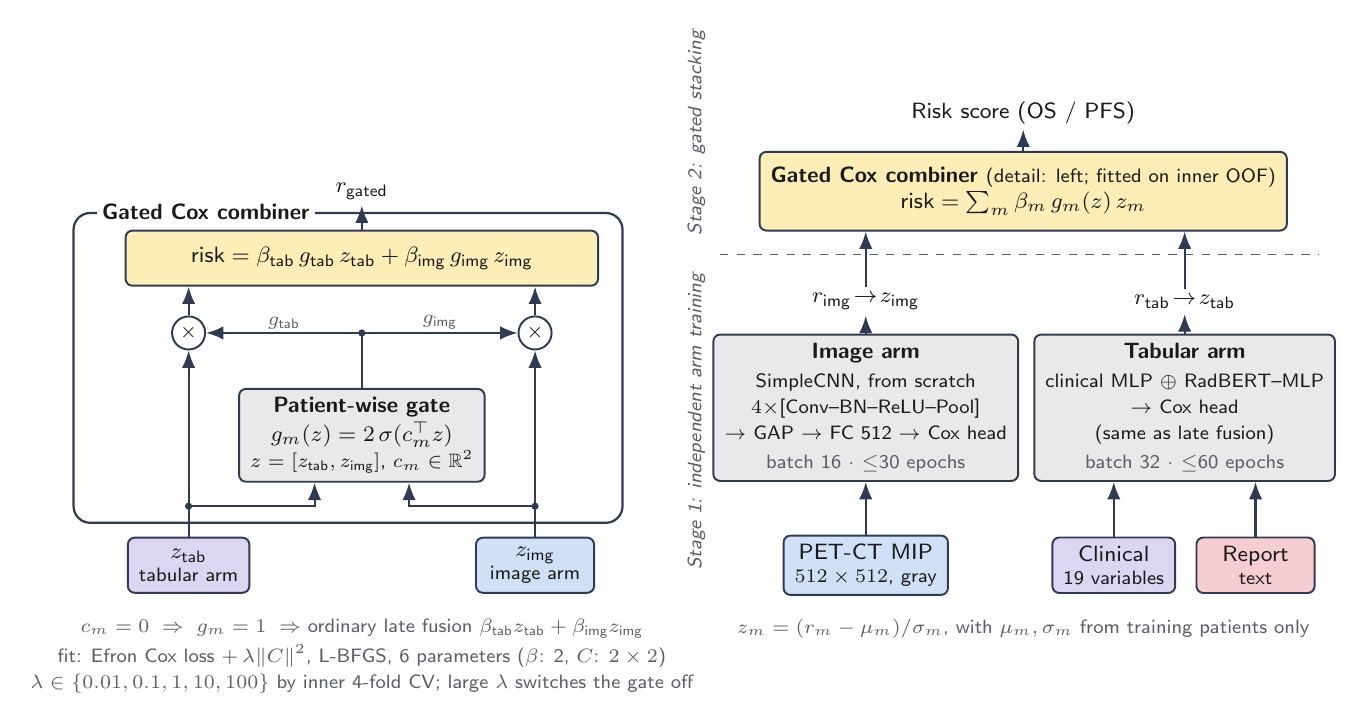
\begin{tikzpicture}[x=1cm,y=1cm]

% ===================== LEFT: gated Cox combiner (detail) =====================
\begin{scope}[shift={(0,0)}]
  % inputs: standardised risk scores
  \node[inp=boxpurple] (zt) at (0,0)   {$z_{\text{tab}}$\\[-1pt]{\scriptsize tabular arm}};
  \node[inp=boxblue]   (zi) at (4.4,0) {$z_{\text{img}}$\\[-1pt]{\scriptsize image arm}};
  % gate
  \node[blk, minimum width=31mm, minimum height=11mm] (gt) at (2.2,1.65)
        {\textbf{Patient-wise gate}\\[1pt] $g_m(z)=2\,\sigma(c_m^{\top}z)$\\ {\scriptsize $z=[z_{\text{tab}},z_{\text{img}}]$, $c_m\in\mathbb{R}^2$}};
  % multiply
  \node[op] (mt) at (0,2.95)   {$\times$};
  \node[op] (mi) at (4.4,2.95) {$\times$};
  % combiner
  \node[blk=boxyellow, minimum width=60mm, minimum height=7mm] (cb) at (2.2,3.9)
        {$\text{risk}=\beta_{\text{tab}}\,g_{\text{tab}}\,z_{\text{tab}}+\beta_{\text{img}}\,g_{\text{img}}\,z_{\text{img}}$};
  \node[risk] (r) at (2.2,4.75) {$r_{\text{gated}}$};
  % arrows: z -> multiply (straight), z -> gate (tap)
  \draw[arr] (zt) -- (mt);  \draw[arr] (zi) -- (mi);
  \fill[navy] (0,0.75) circle (1.3pt);  \fill[navy] (4.4,0.75) circle (1.3pt);
  \draw[arr] (0,0.75) -| ($(gt.south)+(-0.6,0)$);
  \draw[arr] (4.4,0.75) -| ($(gt.south)+(0.6,0)$);
  % gate -> multiply
  \draw[navy, line width=0.75pt] (gt.north) -- (2.2,2.95);
  \fill[navy] (2.2,2.95) circle (1.3pt);
  \draw[arr] (2.2,2.95) -- node[lab, above] {$g_{\text{tab}}$} (mt.east);
  \draw[arr] (2.2,2.95) -- node[lab, above] {$g_{\text{img}}$} (mi.west);
  \draw[arr] (mt.north) -- (mt.north |- cb.south);
  \draw[arr] (mi.north) -- (mi.north |- cb.south);
  \draw[arr] (cb) -- (r);
  % container
  \begin{scope}[on background layer]
    \node[container, fit={(gt)(mt)(mi)(cb)(-1.25,0.75)(5.3,0.75)}] (gc) {};
  \end{scope}
  \node[font=\footnotesize\bfseries, fill=white, inner sep=2pt, anchor=west]
        at ($(gc.north west)+(0.3,0)$) {Gated Cox combiner};
  \node[lab] at (2.2,-0.8) {$c_m=0\;\Rightarrow\;g_m=1\;\Rightarrow$ ordinary late fusion $\beta_{\text{tab}}z_{\text{tab}}+\beta_{\text{img}}z_{\text{img}}$};
  \node[lab] at (2.2,-1.15) {fit: Efron Cox loss $+\,\lambda\lVert C\rVert^2$, L-BFGS, 6 parameters ($\beta$: 2, $C$: $2\times2$)};
  \node[lab] at (2.2,-1.5) {$\lambda\in\{0.01,0.1,1,10,100\}$ by inner 4-fold CV; large $\lambda$ switches the gate off};
\end{scope}

% ===================== RIGHT: full model =====================
\begin{scope}[shift={(8.6,0)}]
  % inputs
  \node[inp=boxblue]   (im) at (0,0)    {PET-CT MIP\\[-1pt]{\scriptsize $512\times512$, gray}};
  \node[inp=boxpurple] (cl) at (3.15,0) {Clinical\\[-1pt]{\scriptsize 19 variables}};
  \node[inp=boxpink]   (rp) at (4.95,0) {Report\\[-1pt]{\scriptsize text}};
  % arms (Stage 1)
  \node[blk, minimum width=30mm, minimum height=17mm] (ia) at (0,2.0)
        {\textbf{Image arm}\\[1pt] {\scriptsize SimpleCNN, from scratch}\\ {\scriptsize $4\times$[Conv--BN--ReLU--Pool]}\\ {\scriptsize $\to$ GAP $\to$ FC 512 $\to$ Cox head}\\[1pt] {\scriptsize\color{ink2} batch 16 $\cdot$ $\le$30 epochs}};
  \node[blk, minimum width=32mm, minimum height=17mm] (ta) at (4.05,2.0)
        {\textbf{Tabular arm}\\[1pt] {\scriptsize clinical MLP $\oplus$ RadBERT--MLP}\\ {\scriptsize $\to$ Cox head}\\ {\scriptsize (same as late fusion)}\\[1pt] {\scriptsize\color{ink2} batch 32 $\cdot$ $\le$60 epochs}};
  % standardised risk scores
  \node[risk] (zi) at (0,3.35)    {$r_{\text{img}}\!\to\! z_{\text{img}}$};
  \node[risk] (zt) at (4.05,3.35) {$r_{\text{tab}}\!\to\! z_{\text{tab}}$};
  % Stage separator
  \draw[dashed, ink2, line width=0.4pt] (-1.85,3.95) -- (5.75,3.95);
  \node[stage, rotate=90, anchor=east] at (-2.15,3.75) {Stage 1: independent arm training};
  \node[stage, rotate=90, anchor=west] at (-2.15,4.15) {Stage 2: gated stacking};
  % combiner (Stage 2)
  \node[blk=boxyellow, minimum width=62mm, minimum height=10mm] (cb) at (2.0,4.75)
        {\textbf{Gated Cox combiner} {\scriptsize(detail: left; fitted on inner OOF)}\\ $\text{risk}=\sum_m\beta_m\,g_m(z)\,z_m$};
  \node[risk] (out) at (2.0,5.75) {Risk score (OS / PFS)};
  % arrows
  \draw[arr] (im) -- (ia);  \draw[arr] (cl) -- (cl |- ta.south);  \draw[arr] (rp) -- (rp |- ta.south);
  \draw[arr] (ia) -- (zi);  \draw[arr] (ta) -- (zt);
  \draw[arr] (zi.north) -- (zi.north |- cb.south);
  \draw[arr] (zt.north) -- (zt.north |- cb.south);
  \draw[arr] (cb) -- (out);
  \node[lab] at (2.0,-0.8) {$z_m=(r_m-\mu_m)/\sigma_m$, with $\mu_m,\sigma_m$ from training patients only};
\end{scope}

\end{tikzpicture}
\end{document}
